\chapter{The Large Hadron Collider}
\label{chap:lhc}

The Standard Model provides a framework for understanding the fundamental particles (e.g. electrons, quarks) and the underlying forces which govern their behavior (e.g photon exchange between two charged particles). The SM details how these particles interact at the quantum mechanical level and these processes can be tested and probed by observing the results of high-energy particle collisions, reconstructing the initial interaction by means of the final state particles. Nature itself has provided us with a source of collisions in the form of cosmic rays: high-energy H and He nuclei coming from outside the Solar System interact with atoms in the atmosphere (e.g. N, O, Ar) causing showers of exotic particles. A diagram of this phenomena is seen in Figure \ref{fig:cosmicrays}. Indeed, there are many experiments which set out to detect such cosmic ray showers. Here we take a different approach and build machines here on Earth to generate particle collisions, although at not nearly such large energies provided by cosmic rays. The Large Hadron Collider (LHC) is a facility which houses two beams of protons (each beam centimeters in transverse size) running parallel in an underground ring 17 miles in circumference. The protons are accelerated to nearly the speed of light by electric fields and are steered within their circular trajectory using magnetic fields generated by superconducting magnets. A schematic of the complex which houses this machine is seen in the left panel of Figure \ref{fig:lhc}; as seen in the diagram, the LHC is the final machine of a number of stages which each incrementally increase the energy of the protons. There are 5 locations around the ring where the beams are crossed and particle detectors are placed. The right panel of Figure \ref{fig:lhc} shows the LHC complex underground near Geneva, Switzerland.

\begin{figure}[hbp!]
\centering
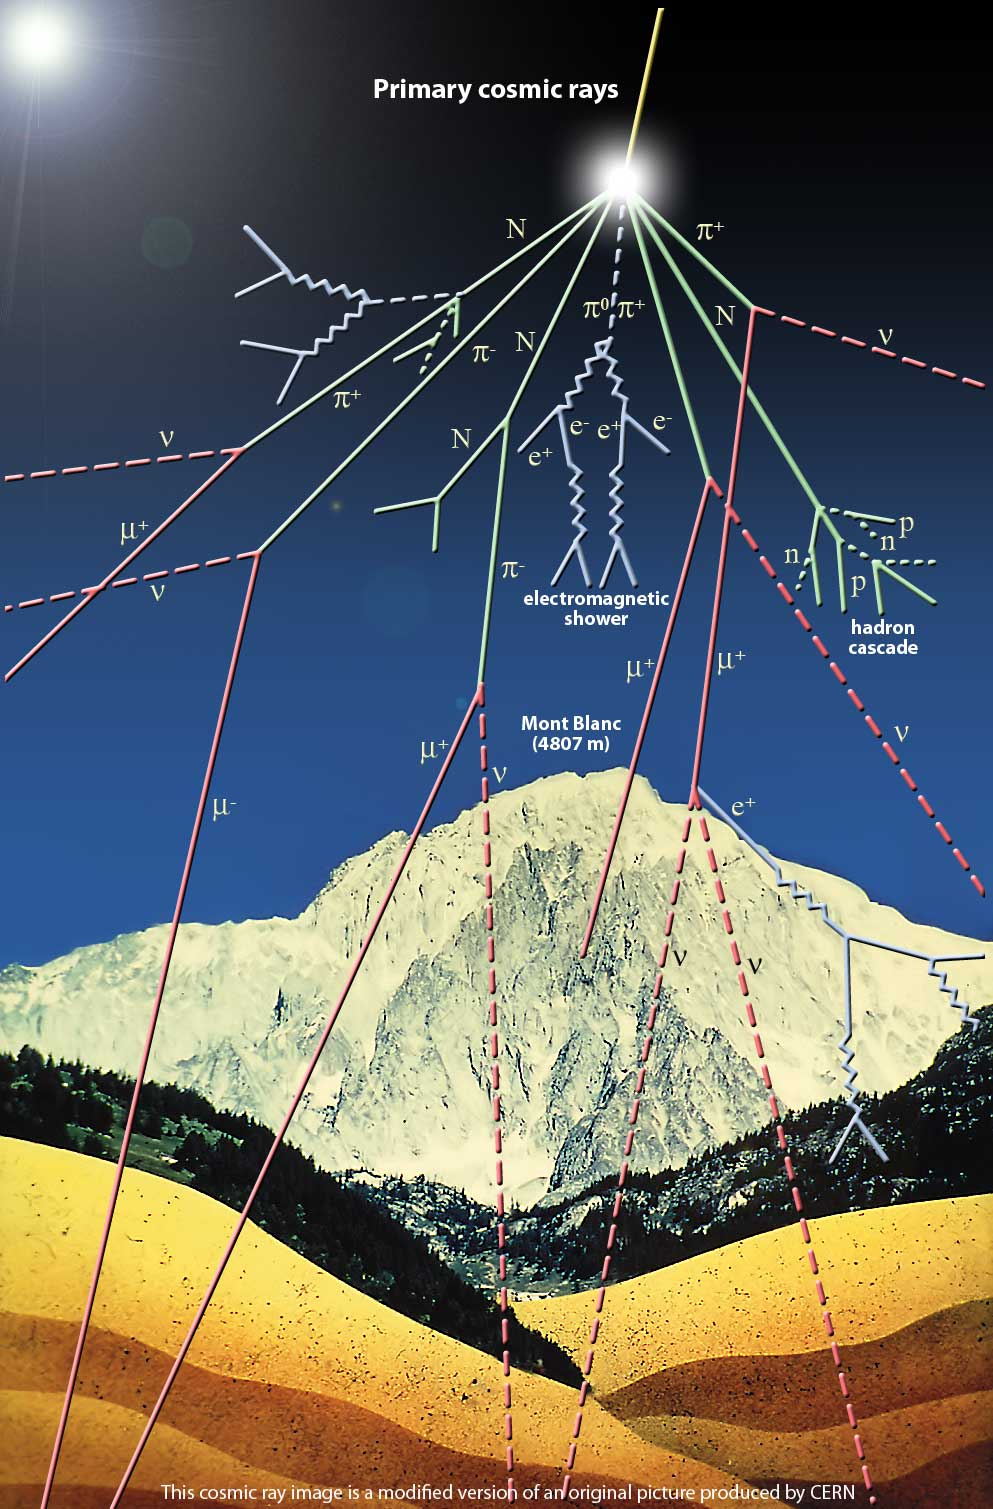
\includegraphics[width=0.45\textwidth]{figs/cosmic-rays.jpg}
\caption{Nature's source of high-energy particle collisions: a cosmic ray shower.}
\label{fig:cosmicrays}
\end{figure}

\begin{figure}[hbp!]
\centering
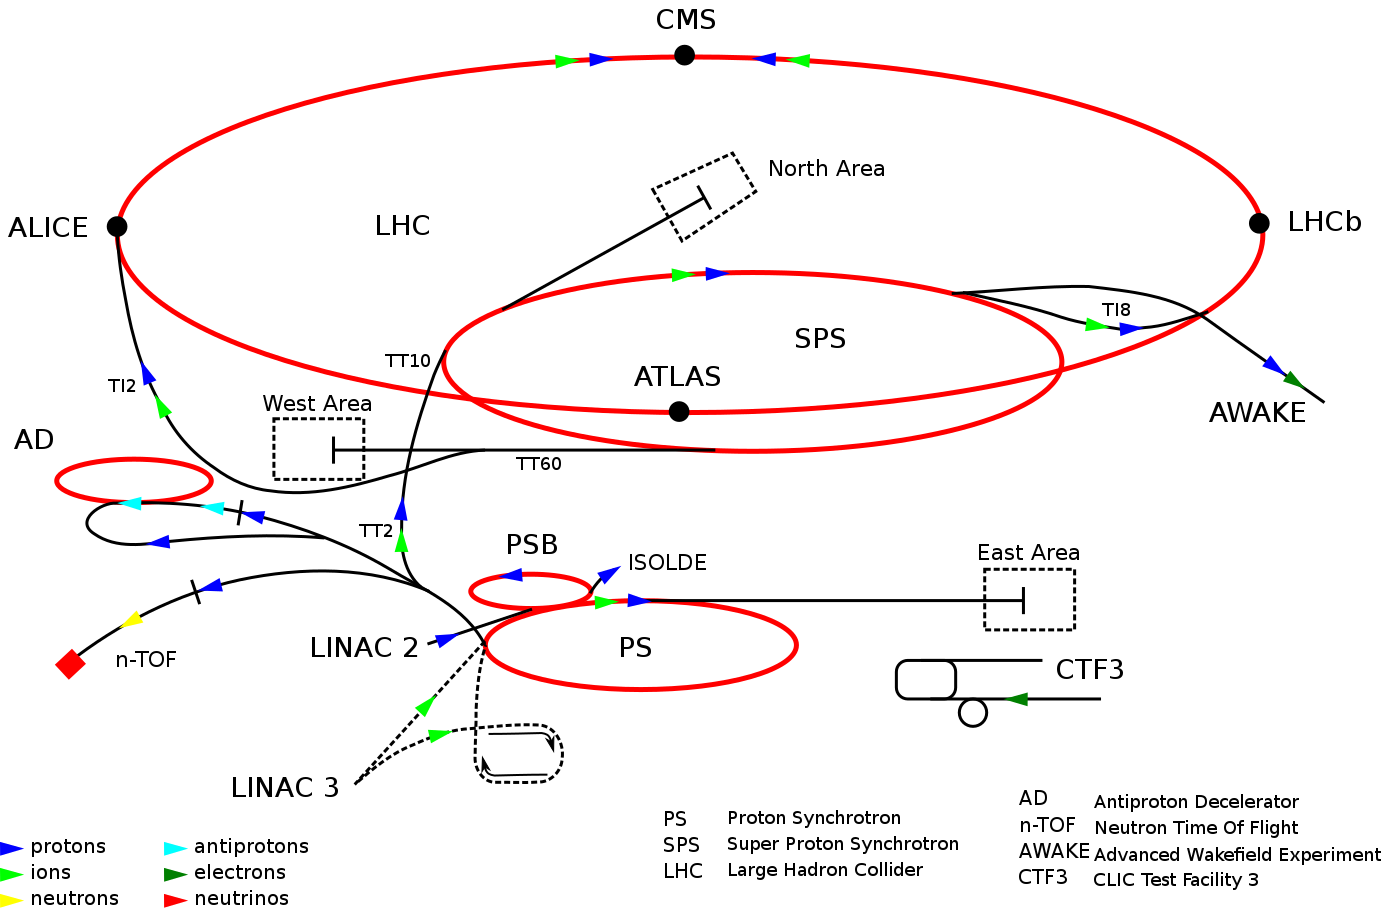
\includegraphics[width=0.55\textwidth]{figs/lhcschematic.png}
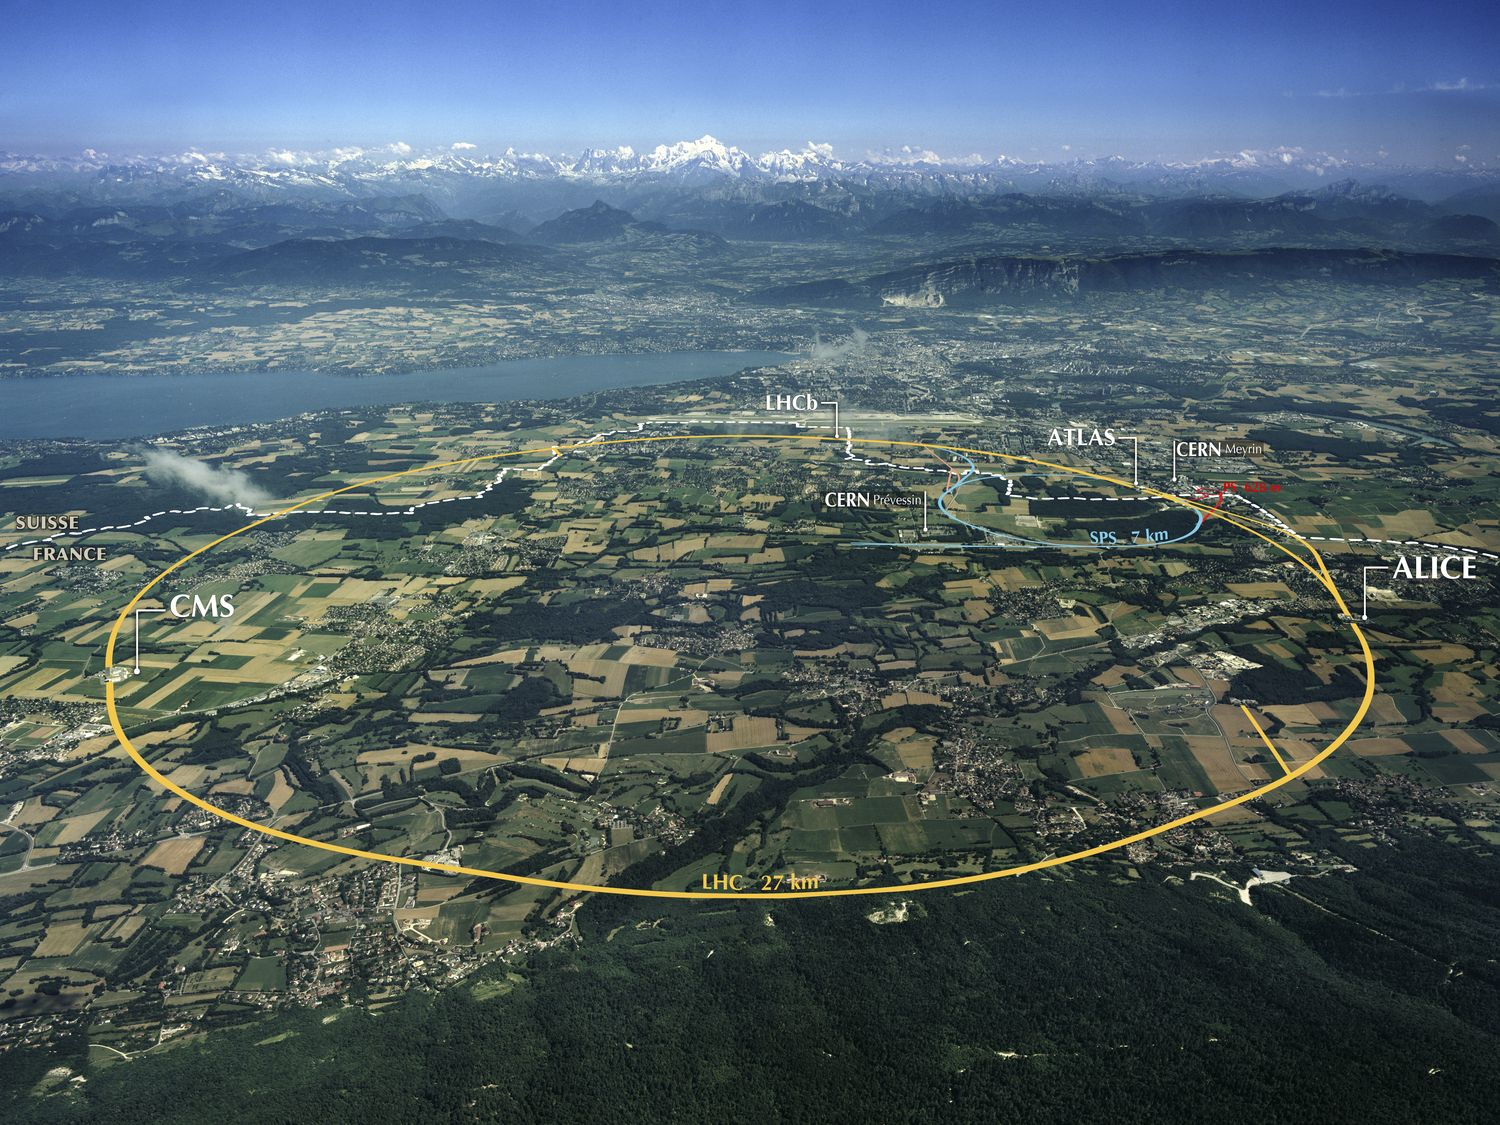
\includegraphics[width=0.4\textwidth]{figs/lhc.jpg}
\caption{The LHC complex; 17 miles around, 500ft underground.}
\label{fig:lhc}
\end{figure}
